
%In many texts however, adaptation is not clearly defined (leading to ambiguity) or is often used in biological irrelevant contexts \citep{Dobzhansky1968}.  
%Even in Darwin's \textit{Origin}, where it is a central concept, adaptation is not explicitly defined throughout the text \citep{darwin1859origin}.
In this section, I will start with the definition of the concepts of adaptation (although there are more than one definitions of adaptation; \citealp{endler1986natural}), and natural selection. Then I will introduce some of the methods that are used to estimate adaptation, with a focus on molecular methods.

\subsubsection{On the concept of adaptation}
%Measuring adaptation is a central theme in evolutionary biology.
Usually adaptation refer to two different things, to an adaptive trait or to the process to become adapted \citep{endler1986natural}.
George Gaylord \citet{Simpson1953} defined adaptation in the following way: 

"\textit{an} adaptation is a characteristic of an organism advantageous to it or to the conspecific group in which it lives, while adaptation or the process of adaptation is the acquisition within a population of such individual adaptation" (italics by the author)

An adaptation (i.e., an adaptive trait) is usually related to a specific function of the organism. For example, the beak variations (in size, width and depth) in the Darwin's Galapagos finches, a classic example of adaptive traits, are related to the alimentary function of the finches, so that each species is specialized in a specific diet.
The notion of adaptation existed before Darwin, but since Darwin it is closely related to the concept of natural selection. Under the current evolutionary framework, an adaptation, arising due to intrinsic natural variation, will be fixed in a population by natural selection due to the advantage it confers to their bearer organisms.

%We say an organism is adapted to an environment when it is able to live and reproduce in it. A related concept is adaptedness, or "the degree to which an organism is adapted to an environment" \citep{Dobzhansky1968}.
%
%In here, I refer to adaptation as a phenotypic character (or modification in a phenotypic character) that arise by natural selection in response to the environment, or other external factor.
%
%Since Darwin, the concepts of adaptation and natural selection usually come together. There has been a long standing controversy on the relationship between natural selection and adaptation.
%For some authors like Barton et al., adaptation is "a trait that functions to increase fitness and that evolved for that function" and that can be only caused by natural selection (REF Barton).
%Other authors however, consider that an adaptation might originate only by chance and natural selection only addresses the spread of adaptive variants (Williams, Gould and Vrba, Alberch).


\subsubsection{Natural selection}

Charles Darwin, in its 1859's \textit{Origin}, defined Natural selection as follows:
%%%%%%%%%%%%%%%%%%%%%%%%%%%%%%%%%%%%%%%%%%%%%%%%%%%%%%%%%%%%%%%%%%%%%%%%%%%%%%%%%%%
\begin{flushleft}
\leftskip3em
\rightskip\leftskip
\footnotesize{
\textit{
" Owing to this struggle (for life), variations, however slight and from whatever cause proceeding, if they be in any degree profitable to the individuals of a species (...) will tend to the preservation of such individuals, and will generally be inherited by the offspring. The offspring, also, will thus have a better chance of surviving, for, of the many individuals of any species which are periodically born, but a small number can survive. I have called this principle,
by which each slight variation, if useful, is preserved, by the term Natural Selection"} \citep{darwin1859origin}.
}
\end{flushleft}
%%%%%%%%%%%%%%%%%%%%%%%%%%%%%%%%%%%%%%%%%%%%%%%%%%%%%%%%%%%%%%%%%%%%%%%%%%%%%%%%%%%

More recently, and following the Darwininan concept of natural selection, Jhon A. \citet{endler1986natural}, defined it as a process in which, given that a population has:

\vspace{3mm}
%%%%%%%%%%%%%%%%%%%%%%%%%%%%%%%%%%%%%%%%%%%%%%%%%%%%%%%%%%%%%%%%%%%%%%%%%%%%%%%%%%%%%%%
\begin{enumerate}[label=\textit{\alph*.}]
\item \textbf{variation} among individuals in some attribute or trait;
\item \textbf{fitness differences} (consistent relationship between that trait and mating ability, fertilizing ability, fertility, fecundity, and, or, survivorship);
\item  \textbf{inheritance} (consistent relationship, for that trait, between parents and their offspring, which is at least partially independent of common environmental effects).
\end{enumerate}
%%%%%%%%%%%%%%%%%%%%%%%%%%%%%%%%%%%%%%%%%%%%%%%%%%%%%%%%%%%%%%%%%%%%%%%%%%%%%%%%%%%%%%%
\vspace{3mm}
Then:
\vspace{3mm}
%%%%%%%%%%%%%%%%%%%%%%%%%%%%%%%%%%%%%%%%%%%%%%%%%%%%%%%%%%%%%%%%%%%%%%%%%%%%%%%%%%%%%%%
\begin{enumerate}
\item the trait frequency distribution will differ among age classes or life-history stages, beyond that expected from ontogeny;
\item\ if the population is not at equilibrium, then the trait distribution of all offspring in the population will be predictably different from that of all parents, beyond that expected
from conditions a and c alone.
\end{enumerate}
%%%%%%%%%%%%%%%%%%%%%%%%%%%%%%%%%%%%%%%%%%%%%%%%%%%%%%%%%%%%%%%%%%%%%%%%%%%%%%%%%%%%%%%
\vspace{3mm}

Conditions a, b, and c are necessary and sufficient for the process of natural selection to occur, and these lead to deductions i and ii \citep{endler1986natural}.

Condition a relates to phenotypic changes across generations. Importantly, phenotypic changes, whether new characters or modifications of existing characters in the adult/larva, are produced from changes in development.
For example, the difference in the beak size and shape between the famous Galapagos Darwin's finches, a classic example of adaptive change under natural selection, has been shown to be regulated by the differential expression of the genes CaM and BMP4 during development \citep{Abzhanov2006}.

Therefore, even when natural selection acts in the adult/larva phenotype, the changes that lead to an adaptation should be traceable during the development of such trait.

\subsubsection{Methods to detect natural selection}

There are many different methods designed to detect natural selection in natural populations. Jhon A. Endler classified ten different methods with diverse ability to detect natural selection \citep{endler1986natural}. Some of these methods test directly the conditions (b and c) required by natural selection, while others test the predicted outcome of natural selection in a population.

There are many studies that have aimed to detect natural selection directly in the phenotype. Usually, these studies are based on the estimation of selection gradients of a quantitative trait (a measurable phenotype that usually depends on the cumulative actions of many genes and the environment). A selection gradient of a trait refers to the relation of the trait values and fitness. Is calculated as the slope of a linear regression of fitness on the trait value \citep{barton2007evolution}.
Most of these studies are based on the analysis a single trait or a small number of traits of an organism \citep{Hoekstra2001,Hereford2004} which are usually selected already under the suspicion to be adaptive. On the contrary, there is practically no study that has attempted to estimate natural selection over the entire organism.

Among the methods that test the predicted outcome of natural selection we find the molecular methods. The molecular methods are based on the assumption that given that changes leading to an adaptation are (at least partially) caused by DNA mutations, the effects of natural selection could be traceable looking at the DNA sequence.
There is an entire field within evolutionary biology, namely molecular evolution, dedicated to explain the sequence changes in molecules as DNA, RNA and proteins in evolution
	\nomenclature{DNA}{Deoxyribonucleic acid}
	\nomenclature{RNA}{Ribonucleic acid}

In the next sections, due to its relevance in this work I will only focus on the molecular methods to detect natural selection.

\subsection{Molecular evolution}

The theoretical basis of the molecular evolution field includes concepts from evolutionary biology and population genetics. At the DNA level, any transmissible change in the sequence is considered a mutation. 
The most simple change is a point mutation, also called single nucleotide polymorphism (SNP),
	\nomenclature{SNP}{Single nucleotide polymorphism} 
which is a change in a single nucleotide in the DNA sequence of a locus in an individual.

Variation at a particular DNA site within the individuals of a species or population is referred as polymorphism, while divergence refers to variation at a specific DNA site in individuals from different species.

SNPs occur in non-coding and coding DNA sequences. A SNP that occurs in a coding sequence is classified in two categories, depending on its effect on the protein sequence: i) synonymous mutation and ii) non-synonymous mutation.
A synonymous mutation does not affect the amino-acid sequence of the protein (although it can affect its function 
	\citep{Kimchi-Sarfaty2007} or the gene transcriptional efficiency \citep{Xia1996}.
A non-synonymous mutation affects the amino-acid sequence of the protein whether by changing a single amino-acid (missense mutation) or by producing a stop codon (non-sense mutation) which results in a truncated version of the protein.

As the non-synonymous mutations can affect dramatically the structure and function of the protein, it would be expected that most non-synonymous mutations have a negative fitness effect.
However, it is also expected that a fraction of non-synonymous mutations, or adaptive substitutions, would have a positive fitness effect that (depending on the strength of the fitness effect and several population genetics parameters) could lead to the fixation of that mutation in the population.

An important branch of the molecular evolution field is dedicated to the identification of adaptive substitutions in a species, which has lead to the development of many statistical tests. 
Importantly, these tests are based on the neutral theory of evolution, proposed by Kimura
	\citep{Kimura1968}.

\subsubsection{Neutral theory of evolution}
In 1968, Mooto Kimura calculated the average rate of nucleotide substitutions in the evolutionary history of mammals.
The result of his calculations was that, on average, one nucleotide has been substituted every 2 years.
For him, this very high rate of substitution was only explainable if most mutations were almost neutral in natural selection 
	\citep{Kimura1968}.
which was in contrast with the prevailing view at the time that practically no mutations were neutral.

In 1969, Kimura proposed that the majority of amino acid substitutions that occurred in proteins are the result of random fixation of selectively neutral or nearly neutral mutations  \citep{Kimura1969}. In the same year, King and Jukes \citep{King1969} proposed independently practically the same hypothesis.

Two important assumptions of the neutral theory of molecular evolution were:

%%%%%%%%%%%%%%%%%%%%%%%%%%%%%%%%%%%%%%%%%%%%%%%%%%%%%%%%%%%%%%%%%%%%%%%%%%%%%%%%%%%%%%%
\begin{enumerate}
\item Deleterious and adaptive mutations are rapidly purged and fixed in a population respectively.
\item Polymorphism is a transitory phase between random fixation or extinction due to genetic drift.
\end{enumerate}
%%%%%%%%%%%%%%%%%%%%%%%%%%%%%%%%%%%%%%%%%%%%%%%%%%%%%%%%%%%%%%%%%%%%%%%%%%%%%%%%%%%%%%%

Importantly, the neutral theory provided a set of testable predictions, providing a null-hypothesis for adaptive molecular evolution.
%This allowed the development of statistical methods to detect adaptive changes.
%i.e., we can say that a sequence has been under positive selection if the amount of changes exceeds the number of changes expected only by neutral evolution.
%Since the 1990's one of the most popular tests has been the McDonald-Kreitman test (MKT), which estimates the proportion of the adaptive substitution resulted from natural selection.

\subsubsection{From neutral to nearly neutral theories}

In the subsequent decades after the proposal of the neutral theory of molecular evolution, much more protein sequence data became available, which made evident the great variation in the evolution rate of proteins.
To account for this, Kimura and Ohta stated that "functionally less important molecules or parts of a molecule evolve faster than more important ones" \citep{Kimura1974}.
Then, Ohta propose that slightly deleterious mutations might be common in amino acid substitutions \citep{Ohta1973}. Later, it was proposed that half of the protein substitutions would be advantageous and the other half deleterious \citep{gillespie1994causes}.
Therefore, the neutral model was replaced by a nearly neutral model with only deleterious substitutions, which in turn was replaced by one with a mixture of positive and negative effects \citep{Ohta1996}.

At the end of the 1970's comparative analyses of protein sequence data began to be replaced for analyses on DNA sequence data, which revealed that synonymous substitutions within coding regions are more frequent than non synonymous (those that change an amino acid) substitutions.
%
From the early 1990s, the expectations of the nearly neutral theory at the DNA sequence level are that substitutions in non coding DNA and synonymous substitutions in coding regions are neutral and amino acid substitutions can be deleterious, neutral or advantageous \citep{Ohta1996}. Statistical methods were then devised to test such expectations.

\subsection{Estimating adaptation at the molecular level}
One of the most popular tests to estimate adaptation at the molecular level has been the McDonald-Kreitman test (MKT), which is used to detect adaptive substitutions comparing the relative numbers of synonymous and non-synonymous differences within a species with those numbers between closely related species.

\subsubsection{McDonald-Kreitman test}

\nomenclature{MKT}{MacDonald-Kreitman test}

John H. McDonald and Martin Kreitman developed this test in 1991 when analysing the divergence in the Alcohol dehydrogenase (Adh) locus in three \textit{Drosophila} species	\citep{McDonald1991}. 
%
The main assumption of the MKT is that the substitutions in a protein are neutral if the inter-specific ratio of non-synonymous ($Dn$) to synonymous ($Ds$) changes is equal to the intra-specific ratio of non-synonymous ($Pn$) to synonymous ($Ps$) changes (i.e. $Dn/Ds = Pn/Ps$).
Any departure from this equality would imply the action of positive or negative selection.
%
Importantly, MKT assumes for simplicity that non-synonymous mutations are either strongly deleterious, neutral or strongly advantageous \citep{McDonald1991}.
%
%Mutations under positive selection therefore would be expected to spread through a population rapidly so they would not contribute to polymorphism but only to divergence substitutions.

In other words, this method assumes that a protein in a given phylogeny has a specific substitution rate for synonymous and another for non-synonymous substitutions. Therefore, when comparing two proteins from two different species that have evolved under neutral conditions, the \textit{total} number of each type of substitutions would depend on the time since the separation between species. If the proteins are from individuals from the same species, it would depend on the time elapsed since the separation of the within-species branches of the phylogeny.
However, the ratio of non-synonymous to synonymous substitutions is expected to be the same in both inter-specific and intra-specific cases. 
In the case of non-synonymous mutations under positive selection (synonymous mutations are expected to be always neutral), the equality of these ratios would disappear. As mutations under positive selection are expected to spread through a population rapidly (and are not expected to very common) they are not expected to be present as polymorphic (i.e., inter-specific) variation, but only as divergent (i.e., inter-specif) one.

Therefore, in the presence of mutations under positive selection, the ratio of non-synonymous to synonymous variation within species should be lower than the ratio of non-synonymous to synonymous variation between species (i.e. $Dn/Ds > Pn/Ps$; see Fig. \ref{fig:MKT}). 
On the contrary, if the observed ratio of non-synonymous to synonymous variation between species is lower than the ratio of non-synonymous to synonymous variation within species (i.e., $Dn/Ds < Pn/Ps$) then negative selection is at work.
	\nomenclature{$Dn$}{Non-synonymous (inter-specific) divergence per site}
	\nomenclature{$Ds$}{Synonymous (inter-specific) divergence per site}
	\nomenclature{$Pn$}{Synonymous (intra-specific) polymorphism per site}
	\nomenclature{$Ps$}{Synonymous (intra-specific) polymorphism per site}
%

%%%%%%%%%%%%%%%%%%%%%%%%%%%%%%%%%%%%%%%%%%%%%%%%%%%%%%%%%%%%%%%%%%%%%
\begin{figure}[h]
  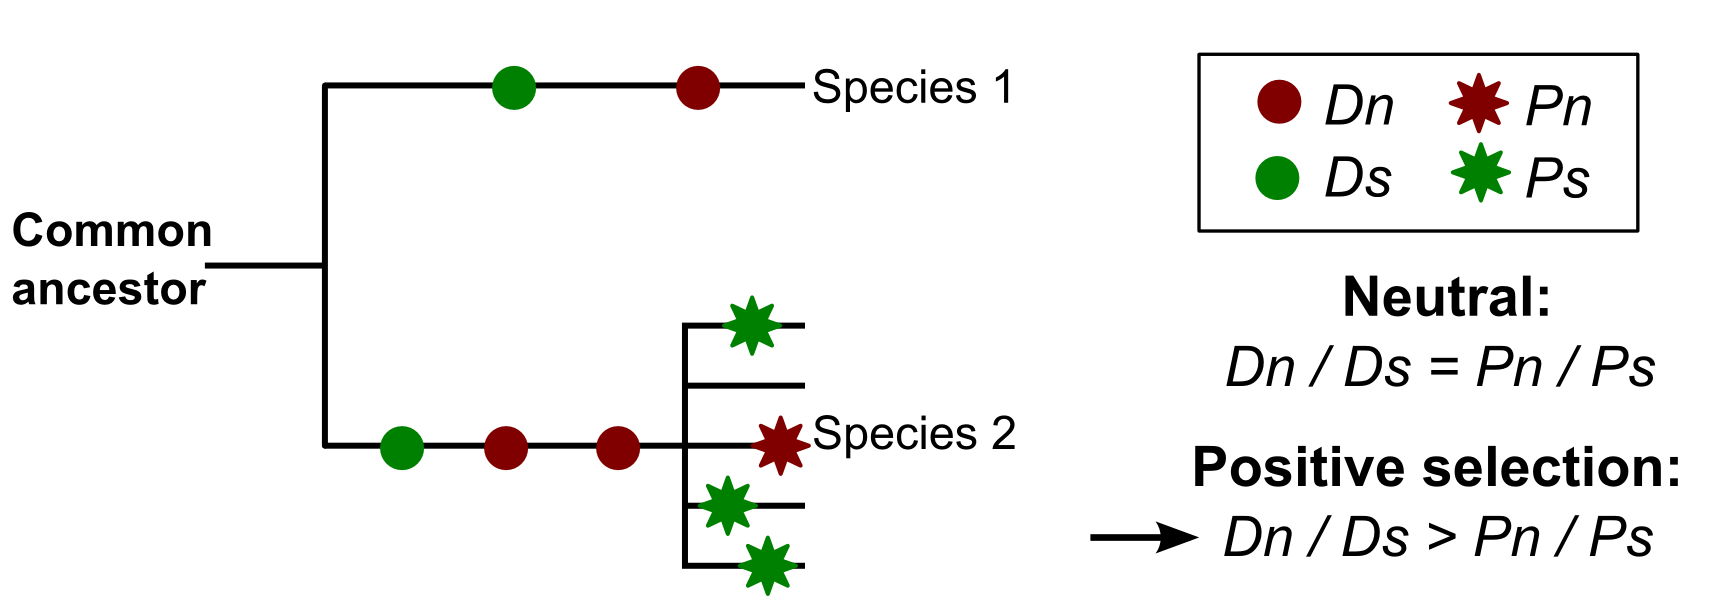
\includegraphics[width=10cm]{./Images/MKT.png}
  \centering
  \caption{\textbf{McDonald-Kreitman Test (MKT).} MKT compares the ratio of non-synonymous ($Dn$; red circle) to synonymous ($Ds$; green circle) divergence ($Dn/Ds$) to the ratio of non-synonymous ($Pn$; red star) to synonymous ($Ps$; green star) polymorphic changes ($Pn/Ps$). Positive selection is detected when $Dn/Ds > Pn/Ps$, as in the example shown in the left.
   }
  \label{fig:MKT}
\end{figure}
%%%%%%%%%%%%%%%%%%%%%%%%%%%%%%%%%%%%%%%%%%%%%%%%%%%%%%%%%%%%%%%%%%%%%

Although the MKT has been proved robust to many sources of error (e.g., variation to mutation rate across the genome), it can be affected by the presence of slightly deleterious mutations or demography \citep{Messer2013,Eyre-Walker2006a}. 
%
The effect of slightly deleterious mutations are related to the effective population size ($N_{e}$). In a population with a low $N_{e}$, slightly deleterious mutations would have more probabilities of fixation by random genetic drift contributing more to polymorphism than to divergence, underestimating the proportion of adaptive changes \citep{Messer2013}.

Recently, sophisticated methods based on the MKT have been developed to correct for underestimation of adaptive evolution in the presence of slightly deleterious mutations. 


\subsubsection{Distribution of Fitness Effects}

%To have a more precise estimate of the proportion of adaptive substitutions it is important to consider the relative contributions of the different types of mutations, based on their fitness effects.
Even when for simplicity the mutation effects are usually classified in strongly advantageous, neutral, and strongly deleterious, there is actually a continuum of selective effects, from strongly deleterious, 
to highly adaptive mutations, with weakly deleterious, neutral and slightly adaptive mutations in between \citep{Eyre-Walker2007}.

The relative frequencies of all these types of mutations is called the Distribution of Fitness Effects (DFE).
	\nomenclature{DFE}{Distribution of Fitness Effects}
In order to know the DFE, a few experimental approaches exist. The most direct method is whether to induce \citep{Sanjuan2004} or to collect \citep{MUKAI1964} spontaneous mutations and assay their effects (fitness) in the laboratory.
As it can be expected, these experiments require many generations to gather sufficient data, so these approaches have been used mainly in micro-organisms \citep{Eyre-Walker2007}.
A caveat of these experimental approaches is that, in order to identify the effect of a mutation, its effect has to be detectable in a fitness assay. In fitness assays however, only effects with relatively large effects are usually detected. Therefore, these methods give valuable information for mutations with relatively large effects.

An alternative approach is to infer the DFE by analysing patterns of DNA sequence differences at intra and inter-specific level (polymorphism and divergence respectively).
The methods using this approach rely mainly on two assumptions:
%%%%%%%%%%%%%%%%%%%%%%%%%%%%%%%%%%%%%%%%%%%%%%%%%%%%%%%%%%%%%%%%%%%%%%%%%%%%%%%%%%%%%%%
\begin{enumerate}
\item  the probability that a mutation spreads to a certain frequency in a population (or to fixation) depends on the strength of selection (positive or negative) acting on it.
Severely deleterious mutations have lower probability to reach a high frequency in a population.
\item\ the efficiency of selection depends on the effective population size. 
With a high effective population size, selection is more efficient and a smaller proportion of mutation will behave as effectively neutral.
\end{enumerate}
%%%%%%%%%%%%%%%%%%%%%%%%%%%%%%%%%%%%%%%%%%%%%%%%%%%%%%%%%%%%%%%%%%%%%%%%%%%%%%%%%%%%%%%
%i) the probability that a mutation spreads to a certain freq in a population (or to fixation) depends on the strength of selection (positive or negative) acting on it.
%Severely deleterious mutations have lower probability to reach a high frequency in a population.
%ii) the efficiency of selection depends on the effective population size. 
%With a high effective population size, selection is more efficient and a smaller proportion of mutation will behave as effectively neutral.
%
The "absolute strength" of selection on a mutation is then measured as $N_{e}s$, the product of the effective population size ($N_{e}$) by the selection coefficient ($s$) of the mutation. Mutations with $N_{e}s$ much less than 1 are effectively neutral, while $N_{e}s$ greater than 100 have no chance to appear as polymorphism \citep{Eyre-Walker2007}.
	\nomenclature{$N_{e}$}{Effective population size}
	\nomenclature{$s$}{Selection coefficient}

\subsubsection{DFE-alpha method} \label{alpha}

Eyre-Walker and collaborators proposed a method to estimate both the DFE and the proportion of adaptive nucleotide substitutions ($\alpha$) using polymorphism and divergence data \citep{Eyre-Walker2009}.
More specifically, they use the polymorphism site frequency spectrum (SFS) to estimate the DFE and then use this estimated DFE to estimate the proportion of substitutions under positive selection between species.
	\nomenclature{$\alpha$}{Proportion of adaptive nucleotide substitutions}
	\nomenclature{SFS}{Site Frequency Spectrum}
	
---- \textbf{how from SFS to DFE?}

This method, assumes that there are two types of nucleotide sites: 
i) sites at which all mutations are neutral and ii) sites at which some of the mutations are subject to selection (positive or negative).
Also it is assumed that any new adaptive mutation in a population would not be detected in the polymorphic phase but only in the divergent one (as the advantageous mutations would fix rapidly in a population), and that the DFE can be represented with a gamma distribution (Figure \ref{fig:Gamma}).

%%%%%%%%%%%%%%%%%%%%%%%%%%%%%%%%%%%%%%%%%%%%%%%%%%%%%%%%%%%%%%%%%%%%%
\begin{figure}[h]
  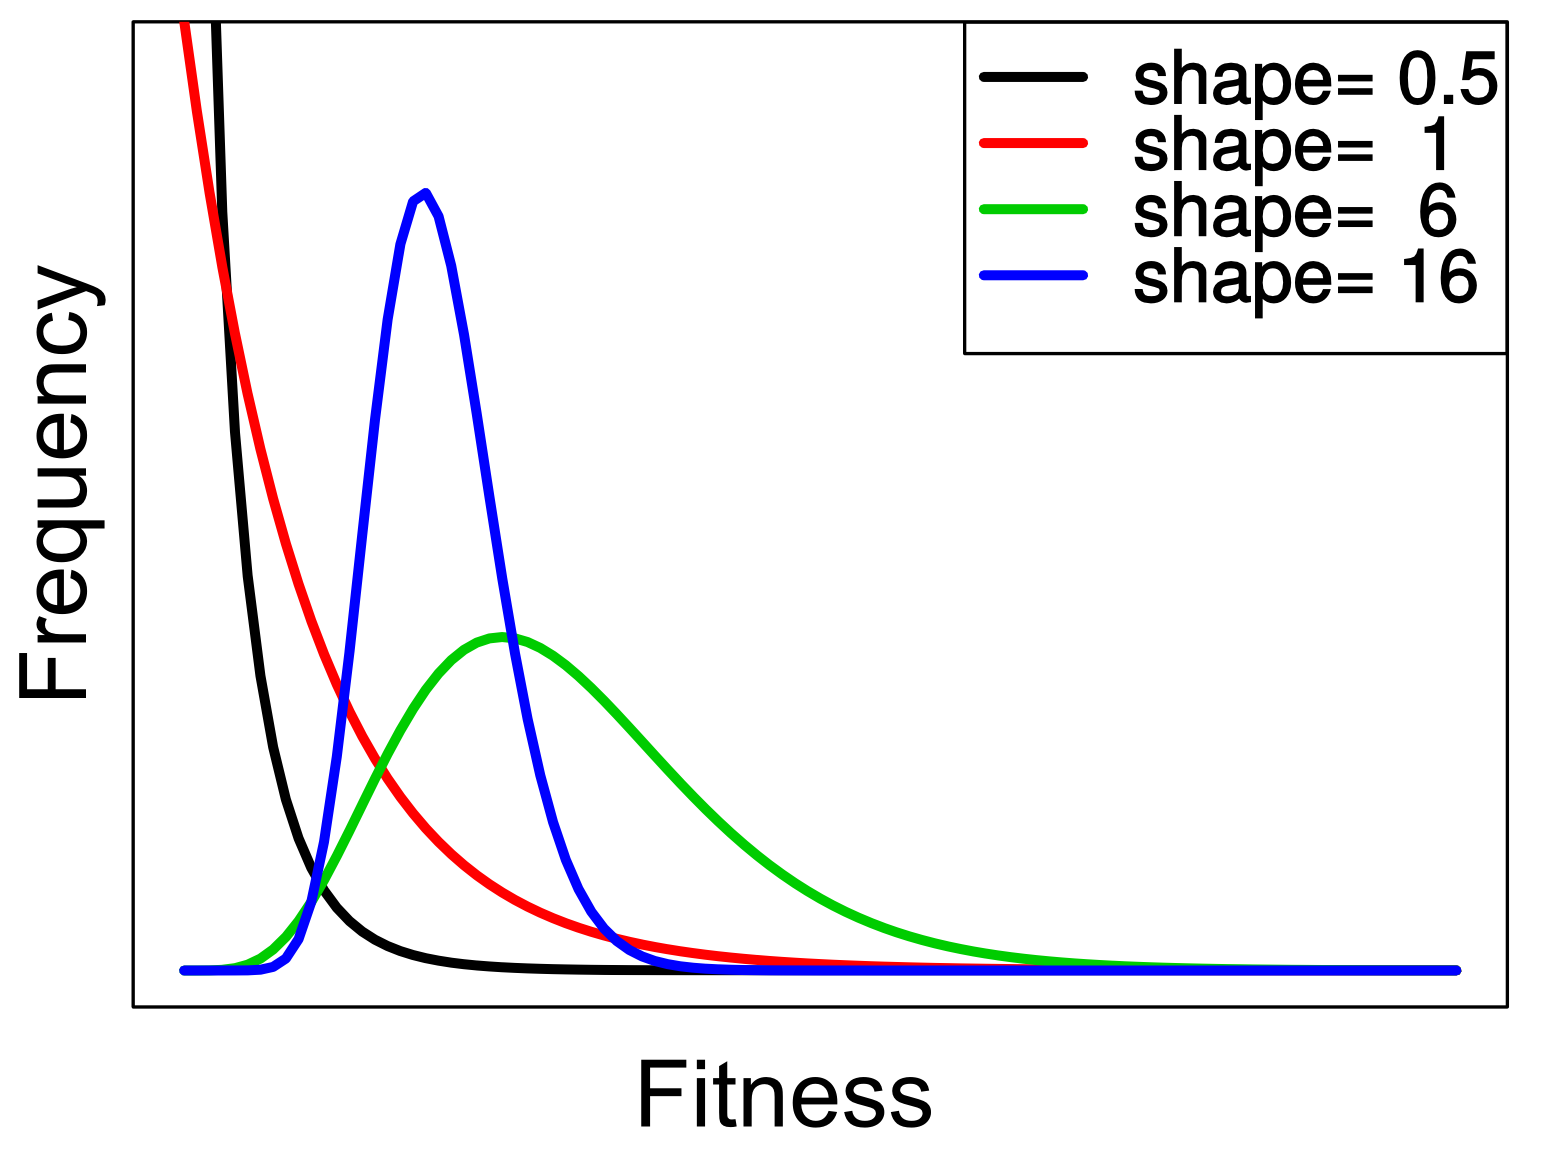
\includegraphics[width=6cm]{./Images/Gamma_dist_2.png}
  \centering
  \caption{Example of different Distribution of Fitness Effects (DFE) represented by a gamma distribution. Many distributions can be represented by modifying the shape parameter of a gamma distribution, from a leptokurtic (shape parameter less than 1) to an exponential (shape parameter equal to 1) or a skewed normal distribution (shape  greater than 1).
   }
  \label{fig:Gamma}
\end{figure}
%%%%%%%%%%%%%%%%%%%%%%%%%%%%%%%%%%%%%%%%%%%%%%%%%%%%%%%%%%%%%%%%%%%%%

The divergence at the neutral sites is then proportional to the mutation rate per site and the predicted divergence at the selected sites (in the absence of advantageous mutations) is proportional to the product of the mutation rate together with the average fixation probability of a selected mutation.
This probability of fixation is is inferred based on the DFE and other parameters estimated from the polymorphism data analysis\citep{Eyre-Walker2009}.
The difference between the observed and predicted divergence therefore estimates the divergence due to adaptive substitutions.
%
Using this method Eyre-Walker and collaborators estimated that approximately 50\% of amino acid substitutions and approximately 20\% of substitutions in introns are adaptive \citep{Eyre-Walker2009}.

Messer and Petrov performed molecular evolution simulations to test if the estimates of different tests, like the MKT and the more sophisticated DFE-alpha, are accurate under different realistic gene-structure and selection scenarios \citep{Messer2013}, specially in the presence of genetic draft (stochastic effects generated by recurrent selective sweeps at closely linked sites)
and background selection (interference among linked sites by lightly deleterious polymorphisms).
%
They found that in the presence of slightly deleterious mutations, MKT estimates of $\alpha$ are severely underestimated and that DFE-alpha is very accurate to calculate $\alpha$ even in the presence of genetic draft, background selection or demography changes \citep{Messer2013}.
%
%This is because genetic draft leaves similar signatures to a recent population expansion, namely distortions of the SFS at synomymous sites, and the DFE-alpha interprets these SFS distortions as being a consequence of demography and attempts to correct for it.
%Importantly, this caveat in using the DFE-alpha is only relevant when demography changes wants to be estimated, but not when alpha is the parameter of interest, as in here.
%
%\subsubsection{Inferring natural selection using a population genomics approach}
%
%For taking advantage of these new methods that infer adaptation combining polymorphism and divergence data, a populations genomics approach is necessary. 
%In the last years, different projects have sequenced, in different species, the genome of many individuals of a population (or a set of populations) \citep{The1000GenomesProjectConsortium2010,Mackay2012,Pool2012,Wallberg2014}, providing a valuable resource of genomic polymorphism data at the population level.
%
%In this study, I used data from the \textit{Drosophila melanogaster} Genetic Reference Panel (DGRP) \citep{Mackay2012}, which consists of inbred \textit{D. melanogaster} lines.
%Importantly, the lines are derived from a single outbred population, so they capture natural variation (as genetic polymorphism) and are ideal to use with methods like the DFE-alpha. 
%
%	\nomenclature{DGRP}{The \textit{Drosophila melanogaster} Genetic Reference Panel}


\subsection{The \textit{Drosophila melanogaster} Genetic Reference Panel} 
\label{DGRP}
	\nomenclature{DGRP}{The \textit{Drosophila melanogaster} Genetic Reference Panel}
In the last years, different population-genomic projects have sequenced, in different species, the genome of many individuals of a population (or a set of populations) \citep{The1000GenomesProjectConsortium2010,Mackay2012,Pool2012,Wallberg2014}, providing a valuable resource of genomic polymorphism data at the population level.
One of these projects is the \textit{Drosophila melanogaster} Genetic Reference Panel (DGRP), a publicly available tool for molecular population genomic analyses.
%
DGRP consists of 192 inbred strains derived from a single outbred \textit{Drosophila melanogaster} population.
The inbred lines were constructed from collected mated females from a Raleigh (North Carolina, USA) population, followed by 20 generations of full-sibling inbreeding of their progeny \citep{Mackay2012}.
168 inbred lines were then sequenced using Illumina (129 lines), 454 sequencing (10 lines) or both (29 lines). Therefore, the DGRP contains a representative sample of naturally segregating genetic variation.

\citealp{Mackay2012} used the DGRP sequence data in combination with genome data from \textit{Drosophila simulans} and \textit{Drosophila yakuba} to analyse polymorphism and divergence, the recombination landscape, and infer the action of natural selection on an unprecedented genome-wide scale.
They found that the patterns of polymorphism differ by autosomal chromosome region, and between the X chromosome and autosomes, contrary to the divergence patterns.
Using version of the MKT test, they estimated that on average 25\% of the fixed sites between \textit{D. melanogaster} and \textit{D. yakuba} are adaptive (24\% non-synonymous, 30\% in introns and 7\% in UTR sites) \citep{Mackay2012}.